%% =====================================================================
%%  Calvin (SIGMOD 2012) -- Analysis of the Scalability Figures
%%  Reconstructed from vector graphics in the original PDF.
%% =====================================================================
\documentclass[11pt,a4paper]{article}

\usepackage[T1]{fontenc}
\usepackage[utf8]{inputenc}
\usepackage{lmodern}
\usepackage[margin=2.4cm]{geometry}
\usepackage{amsmath,amssymb}
\usepackage{booktabs}
\usepackage{siunitx}
\usepackage{array}
\usepackage{longtable}
\usepackage{enumitem}
\usepackage{xcolor}
\usepackage{listings}
\usepackage{float}
\usepackage{caption}
\usepackage{subcaption}
\usepackage{pgfplots}
\usepackage{hyperref}
\usepackage{microtype}

\pgfplotsset{compat=1.18}
\sisetup{group-separator={,}, group-minimum-digits=4}
\setlength{\emergencystretch}{3em}
\hypersetup{colorlinks=true, linkcolor=blue!50!black, citecolor=blue!50!black,
            urlcolor=blue!50!black, pdftitle={Calvin SIGMOD 2012: Analysis of the Scalability Figures}}

\definecolor{calgrayA}{RGB}{204,204,204}
\definecolor{calgrayB}{RGB}{102,102,102}
\definecolor{calblack}{RGB}{0,0,0}

\newcommand{\hot}{C}
\newcommand{\tput}{\ensuremath{X}}
\newcommand{\pernode}{X_m}
\newcommand{\msecs}{\ensuremath{\,\text{\textmu}\text{s}}}
\newcommand{\srcfile}[1]{\texttt{\footnotesize\detokenize{#1}}}
\newcommand{\nueff}{\ensuremath{\nu_{\mathrm{eff}}}}
\newcommand{\gRatio}{g(n)}

\lstdefinestyle{calvin}{
  basicstyle=\ttfamily\footnotesize,
  keywordstyle=\color{blue!50!black}\bfseries,
  commentstyle=\color{gray},
  stringstyle=\color{green!30!black},
  numbers=none,
  frame=single,
  rulecolor=\color{gray!40},
  backgroundcolor=\color{gray!6},
  breaklines=true,
  breakatwhitespace=false,
  xleftmargin=2pt,
  aboveskip=6pt,
  belowskip=8pt,
  showstringspaces=false,
  columns=fullflexible,
  keepspaces=true,
}
\lstset{style=calvin}

\title{\vspace{-1.2cm}\textbf{Analysis of the Scalability Figures in}\\[2pt]
       {\large Calvin: Fast Distributed Transactions for Cloud Databases}\\[6pt]
       \large SIGMOD 2012 \textnormal{---} \small Figure~4 (TPC-C), Figure~5 (microbenchmark), Figure~6 (2PC comparison)}
\author{Data recovered from the vector graphics of the published PDF}
\date{}

\begin{document}
\maketitle
\vspace{-0.6cm}

\begin{abstract}
\noindent
This document analyses the three performance figures in the SIGMOD 2012 Calvin
paper. All numeric values are \emph{digitised} directly from the figures'
PostScript/PDF vector path data (gnuplot output embedded as form XObjects),
calibrated against the axis tick marks and tick labels in the same content
streams; the procedure is documented in Appendix~A and reproduces every
number quoted in the paper's prose to within the stated tolerances.

The analysis establishes six results.
\begin{enumerate}[leftmargin=1.4em,itemsep=2pt]
\item Calvin's scaling is \textbf{linear in aggregate throughput} and
      \textbf{sublinear in per-node throughput}. Per-node throughput
      degrades from a single-node peak to an asymptote, after which total
      throughput grows linearly in $n$ with a constant marginal contribution.
\item The sharp $1\to2$ node knee is caused by \emph{fixed} per-multipartition
      cost, not by any cost that grows with $n$.
\item The \textbf{contention index is scoped per machine}, not globally. The
      system-wide concurrency window is $n/C$, and it is empirically
      demonstrated to be far from binding in every measured configuration.
      A two-part ``global window'' reading of the paper is quantitatively
      \emph{falsified} against the measurement.
\item \textbf{``Distributed transaction'' is not a transaction type.} It is
      never defined in the paper, and inspection of the reference
      implementation (\S\ref{sec:whatis}) shows it is an \emph{emergent
      property of the declared key set}: no component branches on it, the
      participants of a transaction are computed once centrally for routing
      only, and the commit decision is purely local. Being distributed costs
      \num{8.9}--\num{17.3}$\times$ the local work it saves.
\item \textbf{The penalty is not linear in $\rho$, and this falsifies the
      single-$D$ model.} Defining $\gRatio = D(\rho{=}1)/D(\rho{=}0.1)$,
      $\gRatio$ falls sharply from \num{1.561} at $n{=}2$ to
      \num{0.924} at $n{=}100$ (bottoming near \num{0.897} at $n=20$). The
      crossover near $n\approx8$ has a
      clean queueing mechanism (\S\ref{sec:rhonl}) and is not noise.
\item \textbf{There is a second, single-threaded cost centre} that a
      CPU-capacity model misses entirely: the sequencer leader
      deserialises every transaction, computes its participant set, and fans
      it out to $\bar{k}=1+\rho$ sub-batches, all in one thread per replica
      (\S\ref{sec:seq}). It is bounded at $\lesssim\SI{76}{\msecs}$ per extra
      participant, but it exposes a hard ceiling that is independent of
      core count.
\end{enumerate}

\noindent Two results are \emph{weaker than an earlier draft of this
analysis claimed}, and are corrected here: the $1/C$ scaling law
(\S\ref{sec:oneoverC}) was partly absorbing the $\rho$ non-linearity above,
and the attribution of $c_s=\SI{307}{\msecs}$ to eight CPU cores is
unverified --- a single sequencer thread fits the $n{=}1$ data equally well
(\S\ref{sec:nueff}).
\end{abstract}

\tableofcontents
\vspace{2pt}

% =====================================================================
\section{Experimental setup (\S6 of the paper)}
\label{sec:setup}

\begin{table}[H]
\centering
\caption{Testbed and workload configuration. Reproduced from \S6.}
\begin{tabular}{@{}>{\raggedright\arraybackslash}p{3.1cm}
                  >{\raggedright\arraybackslash}p{\dimexpr\textwidth-3.1cm-2\tabcolsep\relax}@{}}
\toprule
\textbf{Property} & \textbf{Value} \\
\midrule
Hardware & Amazon EC2 \texttt{High-CPU/Extra-Large}: \si{7} GiB RAM,
           \si{20} EC2 Compute Units (8 virtual cores $\times$ \si{2.5} ECU),
           $\approx$ one 2007 Opteron/Xeon core per ECU \\
Cluster size & $1 \le n \le 100$ nodes (largest configuration reported) \\
Storage & In-memory key--value store (no disk in these experiments) \\
Replication & None for Figures~4--5; active replication affects only
              latency (Figure~2): \emph{``transactional throughput was
              completely unaffected by changing Calvin's replication mode''} \\
TPC-C (Fig.~4) & New Order transactions only; 10 warehouses per node;
              $\approx10\%$ are multi-warehouse (multipartition) \\
Microbenchmark (Fig.~5) & 10 record reads + constraint check + conditional
              counter updates; tunable contention index and multipartition
              fraction $\rho$ \\
Inter-node latency & $\approx\si{1} ms$ round-trip ping;
              \emph{``one-way latencies $\ldots$ are almost never less than
              \si{2} ms''} \\
Sequencer batching & \emph{``averages \si{5} ms''} \\
\bottomrule
\end{tabular}
\end{table}

\paragraph{Notation.} Throughout, $n$ = node count, $\rho$ = fraction of
transactions that are multipartition, \hot{} = contention index (the paper's
term), $H = 1/\hot{}$ = hot-record set size \emph{per machine},
$\tput$ = aggregate throughput, $\pernode = \tput/n$ = per-node throughput,
$\nu = 8$ = virtual cores per node.

% =====================================================================
\section{Method: recovering the data from vector graphics}
\label{sec:method}

The published figures carry no numeric data labels --- only axis ticks and
gridline-free gnuplot polylines. Every value in this document was therefore
extracted from the raw PDF content streams rather than read off a rendered
image:

\begin{enumerate}[leftmargin=1.4em,itemsep=2pt]
\item Parse the page content stream for path-construction operators
      (\texttt{m}/\texttt{l}) together with stroke-colour operators.
\item Calibrate each axis from the plot frame rectangle and tick marks,
      cross-checked against the tick-label glyph positions extracted with
      \texttt{pdfplumber}.  Agreement is better than \SI{0.3}{\percent}.
\item Group consecutive path operators into polylines; each polyline is one
      data series, identified by its stroke colour.
\item Associate each series with its legend entry by exploiting the
      emission order in the content stream: gnuplot emits the legend key
      line, then the immediately following polyline, then the next key, and
      so on.  This makes the legend mapping unambiguous.
\end{enumerate}

Critically, \texttt{pdfplumber}'s reported coordinates are \emph{incorrect}
for content inside form XObjects (they are off by a non-constant amount), so
the raw streams were parsed directly.  Validation: the reconstructed 1-node
microbenchmark rate is \num{25948} txn/s against the paper's stated
``about \num{27000}''; the 100-node TPC-C rate is \num{440971} against
``nearly half a million''; and the Figure~6 low-contention slowdowns are
$5.4\times$ / $7.0\times$ against the paper's ``\ldots{}from \num{27000} to
about \num{5000} (4 nodes) or \num{4000} (8 nodes)''.

% =====================================================================
\section{Figure 4: TPC-C aggregate scaling}
\label{sec:fig4}

\begin{table}[H]
\centering
\caption{Digitised Figure~4. TPC-C New Order throughput. The two plots in the
figure are the same runs: per-node $=\,$ total$/n$ (verified to
$\le\SI{0.5}{\percent}$).}
\label{tab:fig4}
\begin{tabular}{@{}rrrrr@{}}
\toprule
\textbf{Nodes} & \textbf{Total txn/s} & \textbf{Per-node txn/s} &
\textbf{vs.\ ideal} & \textbf{Marginal txn/s per added node} \\
\midrule
  1  & \num{9570}   & \num{9783}  & \num{9783} & --- \\
  2  & \num{15312}  & \num{7815}  & \num{15630} & \num{5742} \\
  3  & \num{22334}  & \num{7556}  & \num{22668} & \num{7022} \\
  4  & \num{26162}  & \num{6656}  & \num{26624} & \num{3828} \\
  6  & \num{37652}  & \num{6346}  & \num{38076} & \num{5745} \\
  8  & \num{46265}  & \num{5886}  & \num{47088} & \num{4306} \\
 10  & \num{53921}  & \num{5485}  & \num{54850} & \num{3828} \\
 20  & \num{108806} & \num{5524}  & \num{109700} & \num{5489} \\
 30  & \num{149329} & \num{5051}  & \num{151530} & \num{4052} \\
 40  & \num{187938} & \num{4766}  & \num{190640} & \num{3861} \\
 50  & \num{242505} & \num{4922}  & \num{246100} & \num{5457} \\
 60  & \num{289411} & \num{4902}  & \num{294120} & \num{4691} \\
 70  & \num{319084} & \num{4630}  & \num{342100} & \num{2967} \\
 80  & \num{354182} & \num{4494}  & \num{390040} & \num{3510} \\
 \midrule
 100 & \num{440971} & \num{4475}  & \num{478300} & \num{4339} \\
\bottomrule
\end{tabular}
\end{table}

\begin{figure}[H]
\centering
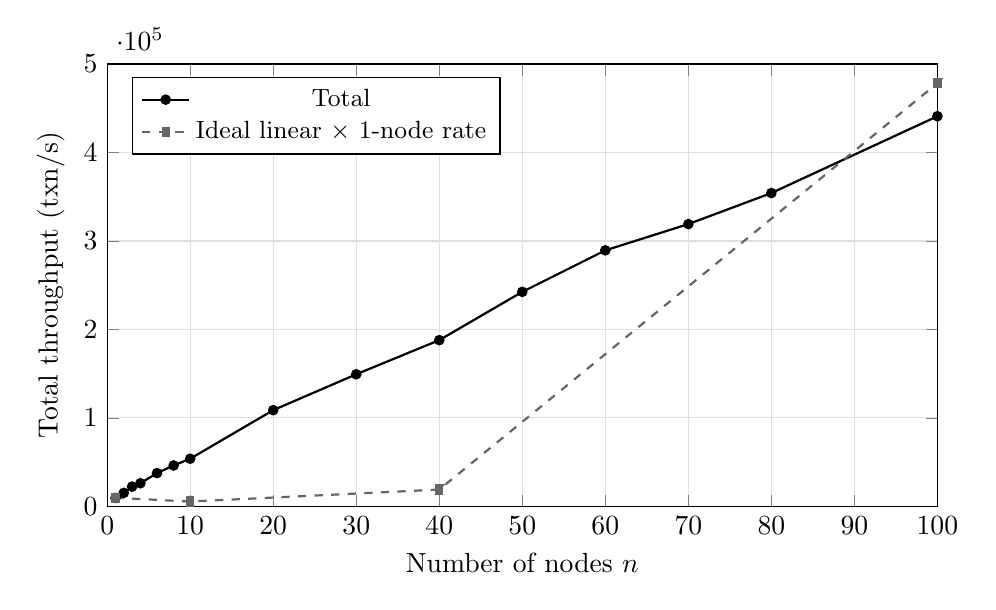
\begin{tikzpicture}
\begin{axis}[
  width=\textwidth, height=7.2cm,
  xlabel={Number of nodes $n$}, ylabel={Total throughput (txn/s)},
  xmin=0, xmax=100, ymin=0, ymax=500000,
  grid=major, grid style={gray!25}, legend style={at={(0.03,0.97)},anchor=north west, font=\small},
]
\addplot[thick, color=calblack, mark=*, mark size=1.5pt]
  coordinates {(1,9570)(2,15312)(3,22334)(4,26162)(6,37652)(8,46265)(10,53921)
               (20,108806)(30,149329)(40,187938)(50,242505)(60,289411)(70,319084)(80,354182)(100,440971)};
\addlegendentry{Total}
\addplot[dashed, color=calgrayB, thick, mark=square*, mark size=1.5pt]
  coordinates {(1,9783)(10,5485)(40,19064)(100,478300)};
\addlegendentry{Ideal linear $\times$ 1-node rate}
\end{axis}
\end{tikzpicture}
\caption{Reconstructed Figure~4 (upper panel). The dashed reference is
$\pernode(1)\times n$; the measured curve tracks it to within
$\approx\SI{8}{\percent}$ at $n=100$, i.e.\ the system runs at
$\approx88\,\%$ of its own post-knee asymptote.}
\label{fig:fig4}
\end{figure}

\subsection*{Three regimes}

\begin{description}[leftmargin=1.2em, itemsep=3pt]
\item[$1\to10$ nodes: the knee.] Per-node throughput falls
      \num{9783} $\to$ \num{5485}, a \SI{44}{\percent} loss.  The paper
      attributes this entirely to \emph{fixed} per-multipartition CPU work,
      which is paid once and then amortised, and therefore does not grow
      with $n$:
      \begin{itemize}[leftmargin=1.2em,itemsep=1pt]
      \item serialising and deserialising remote read results;
      \item additional context switching between transactions blocked on
            remote reads;
      \item set-up, execution and tear-down at \emph{every} participating
            node, \emph{``even though it is counted only once in total
            throughput''}.
      \end{itemize}
\item[$\boldsymbol{n\gtrsim10}$: the plateau.] Per-node throughput is flat
      within \num{4475}--\num{5524} (noise, not trend) and the marginal
      contribution of each added node is a steady
      $\num{4200}$--$\num{5500}$ txn/s.  Aggregate throughput is linear:
      $10\to100$ gives \num{4300}/node, $40\to100$ gives
      \num{4217}/node.
\item[Headline.] \num{440971} New Order txn/s on 100 nodes,
      a $46.1\times$ speedup (\SI{46}{\percent} Amdahl efficiency) but
      $\approx88\,\%$ of the \emph{post-knee} asymptote, since
      $n=1$ already achieves $2.19\times$ the plateau.  The paper compares
      this against Oracle's then-world-record \num{504161} txn/s.
\end{description}

% =====================================================================
\section{Figure 5: the microbenchmark}
\label{sec:fig5}

\subsection{The two panels are one experiment}

\begin{table}[H]
\centering
\caption{Digitised Figure~5. Columns 2--3 are the upper panel; columns 4--5 are
the same points divided by $n$. The identity $\tput(n) = n\cdot\pernode(n)$
holds to $\le\SI{0.5}{\percent}$ (curve~B: \SI{2.6}{\percent}, which contains
two missing x-values).}
\label{tab:fig5}
\begin{tabular}{@{}rrrrrrr@{}}
\toprule
& \multicolumn{2}{c}{\textbf{A: $\rho{=}0.10$, $\hot{=}10^{-4}$}}
& \multicolumn{2}{c}{\textbf{B: $\rho{=}1.00$, $\hot{=}10^{-4}$}}
& \multicolumn{2}{c}{\textbf{C: $\rho{=}0.10$, $\hot{=}10^{-2}$}} \\
\cmidrule(lr){2-3}\cmidrule(lr){4-5}\cmidrule(lr){6-7}
\textbf{$n$} & \textbf{Total} & \textbf{Per-node} & \textbf{Total} &
\textbf{Per-node} & \textbf{Total} & \textbf{Per-node} \\
\midrule
  1 & \num{25948} & \num{26079} & \num{25948} & \num{26029} & \num{25350} & \num{25225} \\
  2 & \num{41644} & \num{20801} & \num{10265} & \num{5268}  & \num{36810} & \num{18328} \\
  3 & \num{60341} & \num{20167} & \num{14488} & \num{4836}  & \num{53702} & \num{17926} \\
  4 & \num{78441} & \num{19645} & \num{19919} & \num{4926}  & \num{68189} & \num{17041} \\
  6 & \num{113445} & \num{18911} & \num{29573} & \num{4956} & \num{101374} & \num{16900} \\
  8 & \num{130337} & \num{16267} & \num{30781} & \num{3810}  & \num{120085} & \num{15010} \\
 10 & \num{155076} & \num{15523} & \num{36212} & \num{3649}  & \num{146033} & \num{14578} \\
 20 & \num{285413} & \num{14266} & \num{62147} & \num{3096}  & \num{232322} & \num{11622} \\
 40 & \num{567213} & \num{14186} & \num{116460} & \num{2915} & \num{322223} & \num{8053} \\
 60 & \num{845389} & \num{14085} & --- & --- & \num{357227} & \num{5952} \\
 80 & \num{1116327} & \num{13954} & --- & --- & \num{415152} & \num{5188} \\
 \midrule
100 & \num{1386654} & \num{13864} & \num{285413} & \num{2855} & \num{474895} & \num{4745} \\
\bottomrule
\end{tabular}
\end{table}

\begin{figure}[H]
\centering
\begin{subfigure}[t]{0.49\textwidth}
\centering
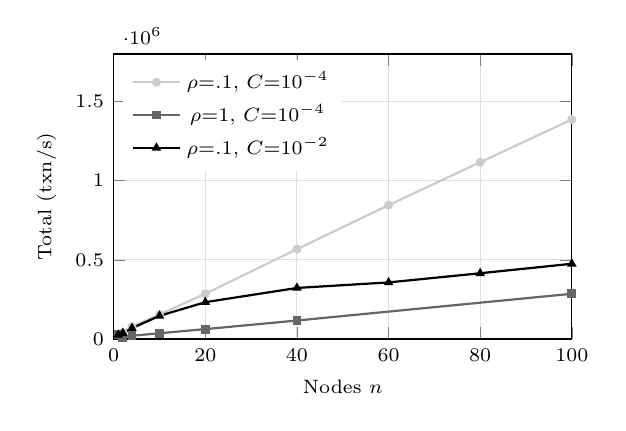
\begin{tikzpicture}
\begin{axis}[width=7.4cm, height=5.2cm,
  xlabel={Nodes $n$}, ylabel={Total (txn/s)},
  tick label style={font=\scriptsize}, label style={font=\scriptsize},
  xmin=0,xmax=100,ymin=0,ymax=1800000, grid=major, grid style={gray!25},
  legend style={at={(0.02,0.98)},anchor=north west,font=\scriptsize,draw=none}]
\addplot[thick,color=calgrayA,mark=*,mark size=1.2pt]
  coordinates {(1,25948)(2,41644)(4,78441)(10,155076)(20,285413)(40,567213)(60,845389)(80,1116327)(100,1386654)};
\addlegendentry{$\rho{=}.1$, $C{=}10^{-4}$}
\addplot[thick,color=calgrayB,mark=square*,mark size=1.2pt]
  coordinates {(1,25948)(2,10265)(4,19919)(10,36212)(20,62147)(40,116460)(100,285413)};
\addlegendentry{$\rho{=}1$, $C{=}10^{-4}$}
\addplot[thick,color=calblack,mark=triangle*,mark size=1.2pt]
  coordinates {(1,25350)(2,36810)(4,68189)(10,146033)(20,232322)(40,322223)(60,357227)(80,415152)(100,474895)};
\addlegendentry{$\rho{=}.1$, $C{=}10^{-2}$}
\end{axis}\end{tikzpicture}
\caption{Total throughput: linear in $n$.}
\end{subfigure}
\hfill
\begin{subfigure}[t]{0.49\textwidth}
\centering
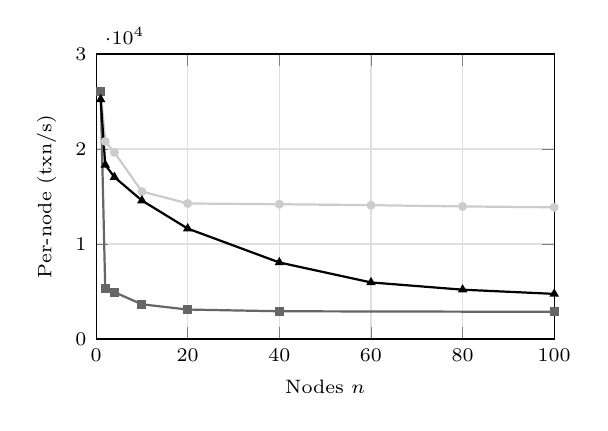
\begin{tikzpicture}
\begin{axis}[width=7.4cm, height=5.2cm,
  xlabel={Nodes $n$}, ylabel={Per-node (txn/s)},
  tick label style={font=\scriptsize}, label style={font=\scriptsize},
  xmin=0,xmax=100,ymin=0,ymax=30000, grid=major, grid style={gray!25}]
\addplot[thick,color=calgrayA,mark=*,mark size=1.2pt]
  coordinates {(1,26079)(2,20801)(4,19645)(10,15523)(20,14266)(40,14186)(60,14085)(80,13954)(100,13864)};
\addplot[thick,color=calgrayB,mark=square*,mark size=1.2pt]
  coordinates {(1,26029)(2,5268)(4,4926)(10,3649)(20,3096)(40,2915)(100,2855)};
\addplot[thick,color=calblack,mark=triangle*,mark size=1.2pt]
  coordinates {(1,25225)(2,18328)(4,17041)(10,14578)(20,11622)(40,8053)(60,5952)(80,5188)(100,4745)};
\end{axis}\end{tikzpicture}
\caption{Per-node throughput $= \tput/n$: same data.}
\end{subfigure}
\caption{Reconstructed Figure~5. A \emph{flat} per-node curve \emph{is} the
signature of linear aggregate scaling, since $\tput = n\cdot\pernode$.}
\label{fig:fig5}
\end{figure}

\subsection*{Marginal throughput: the operational definition of ``linear''}

\begin{table}[H]
\centering
\caption{Aggregate throughput gained per additional node, computed from the
digitised totals. Constant marginal contribution = linear scaling.}
\label{tab:marginal}
\begin{tabular}{@{}lrrr@{}}
\toprule
\textbf{Curve} & \textbf{$10\to100$} & \textbf{$20\to100$} & \textbf{$40\to100$} \\
\midrule
A: $\rho{=}0.10$, $\hot{=}10^{-4}$ & \num{13684} & \num{13765} & \num{13657} \\
B: $\rho{=}1.00$, $\hot{=}10^{-4}$ & \num{2769}  & \num{2791}  & \num{2816}  \\
C: $\rho{=}0.10$, $\hot{=}10^{-2}$ & \num{3654}  & \num{3032}  & \num{2545}  \\
\bottomrule
\end{tabular}
\end{table}

Curve~A is the clean case: the marginal contribution is constant to within
\SI{1}{\percent} across a $10\times$ range of $n$.  Curve~C degrades
(\num{3654} $\to$ \num{2545}) but has not plateaued.

% =====================================================================
\section{The decisive point: the contention index is per-machine}
\label{sec:pernode}

This is the crux, and it is stated \emph{explicitly} in the paper --- twice:

\begin{quote}\small\itshape
``Of the 10 records accessed by the microbenchmark transaction, one is chosen
from a small set of \emph{``hot''} records $\ldots$ except when a
microbenchmark transaction spans two machines, in which case it accesses
\emph{one \emph{``hot''} record on each machine participating} in the
transaction.''
\par\medskip
``\ldots{} we use the term \emph{contention index} to refer to the fraction of
the total \emph{``hot''} records that are updated when a transaction executes
\emph{at a particular machine}.''
\end{quote}

Hence each node owns a private hot set of size $H = 1/\hot$, and a transaction
locks one record from each participating node's set.  The system-wide
concurrency window is therefore

$$\boxed{\;H_{\text{global}} = n \cdot H = \frac{n}{\hot}\;}$$

\noindent\textbf{Consequence.} Holding $\hot$ fixed holds the \emph{per-node}
ceiling fixed. It places no ceiling whatsoever on aggregate throughput, because
each added node contributes its own independent $H$-deep window.

\subsection{Falsification test against the ``global window'' reading}

If instead $\hot$ were read as a \emph{global} window of $H$ concurrent
transactions, then Little's Law gives
$\tput \le H/T_{\text{lock}}$. Using only the paper's own latency floor
($\ge\si{2} ms$ one-way, so $\ge\si{4} ms$ for a remote-read round trip):

\begin{table}[H]
\centering
\caption{The global-window reading is falsified by the measurement.}
\begin{tabular}{@{}>{\raggedright\arraybackslash}p{3.4cm}
                  >{\raggedright\arraybackslash}p{4.5cm}
                  >{\raggedright\arraybackslash}p{\dimexpr\textwidth-7.9cm-4\tabcolsep\relax}@{}}
\toprule
\textbf{Reading of \texorpdfstring{$\hot$}{C}} &
\textbf{Ceiling on $\tput$ at $n{=}100$} & \textbf{Verdict} \\
\midrule
Global, $H{=}1000$ total &
  $\num{1000}/0.004 = \num{250000}$ &
  measured \num{1386654} is $\mathbf{5.5\times}$ \emph{above} this ceiling \\
Per-node, $nH{=}100000$ total &
  $\num{100000}/0.004 = \num{25000000}$ &
  measured is \SI{5.5}{\percent} of this ceiling: consistent \\
\bottomrule
\end{tabular}
\end{table}

Even at an implausibly fast \SI{1} ms round trip the global reading caps out at
\num{1000000} txn/s --- still below the measured \num{1386654}.

\subsection{The window is never binding}

A stronger, assumption-free statement. Applying Little's Law to the hot window,
$\pernode \le H/T_{\text{lock}}$. Taking $T_{\text{lock}} \approx \si{4} ms$
(the paper's own floor plus batching delay):

\begin{table}[H]
\centering
\caption{Implied mean concurrency $h = \pernode \cdot T_{\text{lock}}$ against
the available window $H$. Every configuration is far from saturation.}
\begin{tabular}{@{}lrrrr@{}}
\toprule
\textbf{Curve} & \textbf{$H$} & \textbf{$\pernode$ at $n{=}100$} &
\textbf{Max tolerable $T$} & \textbf{$h$ at $T{=}$4\,ms} \\
\midrule
A: $\rho{=}0.10$, $\hot{=}10^{-4}$ & \num{1000} & \num{13864} & \num{72.1}\,ms & \num{55}\phantom{0} (\SI{5.5}{\percent}) \\
B: $\rho{=}1.00$, $\hot{=}10^{-4}$ & \num{1000} & \num{2855}  & \num{350.3}\,ms & \num{11}\phantom{0} (\SI{1.1}{\percent}) \\
C: $\rho{=}0.10$, $\hot{=}10^{-2}$ & \num{100}  & \num{4745}  & \num{21.1}\,ms & \num{19}\phantom{0} (\SI{19}{\percent}) \\
\bottomrule
\end{tabular}
\end{table}

Every measured point sits $5\times$ to $36\times$ inside its admissible
window. Whatever limits Calvin in these experiments, it is \emph{not} the
contention window --- so the contention window cannot cap anything. The index
is best understood as a \emph{collision-probability} knob (probability that
random transactions collide on one of $H$ records), not a throughput ceiling.

\paragraph{A stronger reason, from the load generator.} The argument above is
circumstantial, because it has to assume a lock-hold time. The reference
implementation removes the need for an assumption: the benchmark client is
co-located with the sequencer and fills each batch as fast as it can inside the
epoch window (\srcfile{sequencer.cc:119}):
\begin{lstlisting}[language=C]
while (!deconstructor_invoked_ &&
       GetTime() < epoch_start + epoch_duration_) {
  if (batch_message.data_size() < max_batch_size_) {
    client_->GetTxn(&txn, ...);   // generate as fast as possible
  } else { usleep(50); }
}
\end{lstlisting}
The load is therefore \textbf{open-loop and rate-unbounded}: concurrency is
\emph{emergent}, chosen by the system, never imposed by a closed-loop client.
A hot-record window can only bind if the system \emph{chooses} to run more
than $H$ transactions in flight --- and it demonstrably does not. This is a
structural guarantee rather than a numerical coincidence.

% =====================================================================
\section{What the paper never defines: the distributed transaction}
\label{sec:whatis}

The phrase appears nine times in the paper's Figure~4 and Figure~5 legends and
in \S1.1, always as a workload knob (``\emph{10\% distributed txns}''), and is
never defined. The paper uses two names for the same thing interchangeably ---
\emph{distributed transaction} (\S1.1, both figure legends) and
\emph{multipartition transaction} (\S6.2, Figure~6) --- and gives only indirect
definitions:

\begin{quote}\small\itshape
``multi-warehouse New Order transactions (about 10\% of total New Order
transactions) \emph{always access a second warehouse that is not on the same
machine as the first}'' (\S6.1)

``except when a microbenchmark transaction \emph{spans two machines}, in which
case it accesses one `hot' record on each machine participating in the
transaction'' (\S6.2)
\end{quote}

So: \textbf{the declared read/write set touches more than one partition.} The
reference implementation makes this precise, and in doing so exposes four
facts that the model in \S\ref{sec:model} must account for.

\subsection{It is not a type; it is a consequence of key selection}

\texttt{MicroTxnMP} in \srcfile{src/applications/microbenchmark.cc:101} takes
\emph{two explicit partition ids} and draws keys from two disjoint ranges:
\begin{lstlisting}[language=C]
uint64 hotkey1 = part1 + nparts * (rand() % hot_records);
uint64 hotkey2 = part2 + nparts * (rand() % hot_records);
// -> read_write_set: one hot key per partition
GetRandomKeys(&keys, kRWSetSize/2 - 1, nparts*hot_records,
                                  nparts*kDBSize, part1);
GetRandomKeys(&keys, kRWSetSize/2 - 1, nparts*hot_records,
                                  nparts*kDBSize, part2);
\end{lstlisting}
No flag is set that says ``distributed''. The client chooses a partner
uniformly at random and the transaction simply spans two ranges
(\srcfile{src/machine/client.h:57}):
\begin{lstlisting}[language=C]
if (nodes_per_replica_ > 1 && (uint32)(rand() % 100) < percent_mp_) {
  do { other = (uint64)(rand() % nodes_per_replica_); }
  while (other == replative_node_id_);
  *txn = microbenchmark.MicroTxnMP(txn_id, rel.ative_node_id_, other);
}
\end{lstlisting}
\texttt{percent\_mp} is literally the Figure~5 legend: \texttt{--percent\_mp=10}
is ``10\% distributed txns''. A search for \texttt{txn\_type} across the whole
tree returns hits \emph{only} under \srcfile{src/applications/} and
\srcfile{src/scripts/}. The sequencer, lock manager, storage manager and
network layer never read it. The single runtime-adjacent read is the
workload's own arithmetic (\srcfile{microbenchmark.cc:473}):
\texttt{if (txn\_type == MICROTXN\_MP) factor = 2.0;} --- a distributed
transaction does twice the deliberate CPU spin per node. That is a benchmark
parameter, not system behaviour.

\subsection{SP and MP transactions have identical size}

\texttt{MicroTxnSP} is $2$ hot $+\,(k_{\text{RW}}-2)$ cold, all local.
\texttt{MicroTxnMP} is $2$ hot $+\,(k_{\text{RW}}/2-1) + (k_{\text{RW}}/2-1)$
cold, split across two nodes. With $k_{\text{RW}}=10$ \emph{both are exactly
ten keys}; the distributed one simply splits them $5/5$.

\textbf{Therefore a distributed transaction halves its local work per node},
yet per-node throughput falls. Decomposing $c_m$ accordingly (using
$c_s=\SI{307}{\msecs}$ from the $n{=}1$ point):

\begin{table}[H]
\centering
\caption{Local work versus distributed overhead, per node per transaction.
Local work is $(1-\rho)c_s+\rho\,c_s/2$.}
\label{tab:overhead}
\begin{tabular}{@{}lrrrr@{}}
\toprule
\textbf{Curve} & \textbf{$n$} & \textbf{$c_m$} & \textbf{local work} &
\textbf{distributed overhead} \\
\midrule
$\rho{=}0.10$ &  2 & \SI{384.6}{\msecs} & \SI{291.7}{\msecs} & \SI{92.9}{\msecs}\phantom{0} (0.3$\times$) \\
$\rho{=}0.10$ & 10 & \SI{515.4}{\msecs} & \SI{291.7}{\msecs} & \SI{223.7}{\msecs}\phantom{0} (0.8$\times$) \\
$\rho{=}0.10$ & 100 & \SI{577.0}{\msecs} & \SI{291.7}{\msecs} & \SI{285.4}{\msecs}\phantom{0} (1.0$\times$) \\
\midrule
$\rho{=}1.00$ &  2 & \SI{1518.6}{\msecs} & \SI{153.5}{\msecs} & \SI{1365.1}{\msecs} (\textbf{8.9$\times$}) \\
$\rho{=}1.00$ & 10 & \SI{2192.4}{\msecs} & \SI{153.5}{\msecs} & \SI{2038.9}{\msecs} (\textbf{13.3$\times$}) \\
$\rho{=}1.00$ & 100 & \SI{2802.1}{\msecs} & \SI{153.5}{\msecs} & \SI{2648.6}{\msecs} (\textbf{17.3$\times$}) \\
\bottomrule
\end{tabular}
\end{table}

The headline number: \textbf{being distributed costs $8.9$--$17.3\times$ the
local work it saves.} The paper attributes this to serialising remote read
results, context switching, and per-participant set-up/tear-down. The code
confirms that list but shows the emphasis is wrong --- serialising five keys is
a few microseconds. The \SI{1365}{\msecs} floor at $n{=}2$ is the
\emph{barrier}: the round trip and the context switch into and out of it.

\subsection{The participant set \emph{is} computed --- centrally, for routing only}

An earlier draft of this analysis asserted that no component establishes which
nodes participate. \textbf{That was wrong.} \texttt{Sequencer::RunReader}
(\srcfile{src/machine/sequencer.cc:187}) computes it, in one thread per
replica:
\begin{lstlisting}[language=C]
for (int i = 0; i < message.data_size(); i++) {
  txn.ParseFromString(message.data(i));
  set<uint64> readers, writers;
  for (read_set)       readers.insert(LookupPartition(key));
  for (read_write_set) { writers.insert(LookupPartition(key));
                         readers.insert(mds); }
  for (r : readers) txn.add_readers(r);
  for (w : writers) txn.add_writers(w);      // == "active participants"

  txn.SerializeToString(&txn_data);          // re-serialise
  for (it : readers) batches[*it].add_data(txn_data);   // fan out, k copies
}
\end{lstlisting}
\texttt{writers} is exactly \S3.2's active participants; \texttt{readers} minus
\texttt{writers} are the passive participants. \texttt{StorageManager} consumes
the lists to assign its own role (\srcfile{storage_manager.cc:20,159}):
\texttt{if (txn->readers(i) == relative\_node\_id\_)} --- am I a reader?
\texttt{if (txn->writers(i) == ...)} --- am I active?

What survives is the substantive point: the lists are used \textbf{only for
routing and role assignment}. The commit decision remains local and
uncoordinated (\srcfile{storage_manager.cc:172}):
\begin{lstlisting}[language=C]
if (involved_machines_.size() == 1) {        // fast path: no peer to ask
  decision = true;
} else {
  for (read_set) if (key_entry.master()   != val->master   ||
                     key_entry.counter() != val->counter) { decision=false; break; }
  // ... and likewise for read_write_set
}
\end{lstlisting}
No round trip, no vote, no participant agreement. Every node reaches the same
verdict independently because the deterministic lock order has already
serialised everything that could conflict. This is the precise sense in which
Calvin escapes the \emph{obligation} of a distributed transaction while
incurring its \emph{cost} --- and it is exactly the premise of \S1.1's
argument, which presupposes a system that must \emph{negotiate}.

% =====================================================================
\section{An analytical model}
\label{sec:model}

\subsection{Formulation}

The naive form of the model is a pure CPU-capacity law: per-node cost is
irreducible single-partition work plus a per-multipartition penalty that
saturates with $n$, and throughput is $\nueff$ divided by that cost.

\begin{align}
c_m(n) &= c_s + \rho \cdot D(n), \label{eq:cost}\\
D(n) &= D_\infty\left(1 - e^{-n/n_0}\right), \label{eq:sat}\\
\pernode(n) &= \frac{\nueff}{c_m(n)}, \qquad
\tput(n) = n\cdot\pernode(n). \label{eq:x}
\end{align}

\begin{itemize}[leftmargin=1.2em,itemsep=2pt]
\item $c_s$: cost of a single-partition transaction. At $n=1$,
      $c_s = \nueff/\pernode(1) = 8/26079 = \SI{307}{\msecs}$.
      \textbf{The attribution of this to eight CPU cores is unverified} ---
      see \S\ref{sec:nueff}.
\item $D(n)$: per-multipartition-transaction penalty.
\item Saturation: a node's reachable window into the global sequence is
      $\sim H/h$ transactions ($h$ = in-flight). Once $n$ is large enough that
      every node holds a full complement of in-flight transactions, adding
      peers adds no further skew exposure, so $D$ saturates and $\pernode$
      plateaus --- making $\tput$ linear in $n$ forever.
\end{itemize}

\subsection{The corrected form}

\S\ref{sec:whatis} forces three changes. \eqref{eq:cost}--\eqref{eq:x} is
retained as the \emph{first-order} description, but the full model has two
ceilings and a decomposed penalty:

\begin{equation}
\boxed{\;
\pernode(n,\rho) = \min\!\left[
\frac{\nueff}{\,c_s+\rho\big(\Delta_{\mathrm{barrier}}
                            + S_\infty(1-e^{-n/n_0})\big)},
\quad
\frac{1}{\,a+(1+\rho)\,b\,}
\right] \;}
\label{eq:corrected}
\end{equation}

\begin{description}[leftmargin=1.4em,itemsep=3pt]
\item[$\Delta_{\mathrm{barrier}}$] The $\rho$-independent floor: one remote
      round trip plus the context switch into and out of it. Constant in $n$.
      Table~\ref{tab:overhead} puts it at $\approx\SI{1365}{\msecs}$.
\item[$S_\infty(1-e^{-n/n_0})$] Execution-progress skew, saturating. This is
      the only genuinely $n$-dependent term, and it is what makes $\pernode$
      plateau.
\item[$a+(1+\rho)b$] The \textbf{single-threaded sequencer ceiling}
      (\S\ref{sec:seq}). One thread per replica deserialises every
      transaction, computes its participant set, re-serialises, and copies it
      into $\bar{k}=1+\rho$ sub-batches. Independent of core count.
\item[$\nueff$] \textbf{Ambiguous}: eight CPU cores, or one sequencer thread?
      \S\ref{sec:nueff} shows the data cannot distinguish them, and this is
      now the largest single uncertainty in the model.
\end{description}

The decomposition into $\Delta_{\mathrm{barrier}}+S_\infty(\cdot)$ was already
flagged as necessary in the original draft's caveats, where the single-$D$ form
failed at $n{=}2$ ($\approx\num{7300}$ predicted vs.\ \num{5268} measured). It
now has a mechanism rather than being an empirical patch: at $n=2$ there is no
accumulated skew, only one round trip.

\subsection{The penalty is not linear in $\rho$}

This is the finding that falsifies \eqref{eq:cost}. That equation requires
$D(\rho{=}1) = 10\,D(\rho{=}0.1)$, since $c_m-c_s$ is linear in $\rho$ by
construction. It is not.

\begin{table}[H]
\centering
\caption{Test of $\rho$-linearity. $D(n) = \bigl(\nueff/\pernode - c_s\bigr)/\rho$
evaluated independently on the two $C=10^{-4}$ curves. If $D$ were
$\rho$-independent, $\gRatio\equiv 1$.}
\label{tab:rhonl}
\begin{tabular}{@{}rrrr@{}}
\toprule
\textbf{$n$} & \textbf{$D(\rho{=}0.1)$} & \textbf{$D(\rho{=}1.0)$} &
\textbf{$\gRatio = D_1/D_{0.1}$} \\
\midrule
  2 & \SI{776.0}{\msecs}  & \SI{1211.6}{\msecs} & \textbf{1.561} \\
  3 & \SI{896.9}{\msecs}  & \SI{1347.3}{\msecs} & 1.502 \\
  4 & \SI{1002.3}{\msecs} & \SI{1317.0}{\msecs} & 1.314 \\
  6 & \SI{1160.3}{\msecs} & \SI{1307.2}{\msecs} & 1.127 \\
  8 & \SI{1847.9}{\msecs} & \SI{1792.7}{\msecs} & 0.970 \\
 10 & \SI{2083.6}{\msecs} & \SI{1885.4}{\msecs} & 0.905 \\
 20 & \SI{2537.7}{\msecs} & \SI{2277.0}{\msecs} & 0.897 \\
 40 & \SI{2569.4}{\msecs} & \SI{2437.4}{\msecs} & 0.949 \\
\midrule
100 & \SI{2700.3}{\msecs} & \SI{2495.1}{\msecs} & \textbf{0.924} \\
\bottomrule
\end{tabular}
\end{table}

$\gRatio$ starts at \num{1.561} and settles at $\approx\num{0.92}$, crossing
unity near $n\approx8$. \textbf{The all-distributed configuration is
substantially more expensive per distributed transaction at small $n$, and
slightly cheaper at large $n$.} This is not noise, and it has a clean
mechanism. Note also that $D$ for $\rho=0.1$ is still climbing at
$n=100$ (\num{2084} $\to$ \num{2700}, $+30\%$) while for $\rho=1$ it has
essentially converged by $n=20$ --- the two curves differ in \emph{shape}, not
just in offset.

\subsection{Why: partner correlation, and it vanishes with $n$}
\label{sec:rhonl}

The client picks the partner uniformly among the $n-1$ other partitions
(\srcfile{client.h:57}). At $n=2$ there is \emph{exactly one} partner, so every
distributed transaction at node $m$ contends for the same fan-out slot and the
same remote-read reply stream: the waits are perfectly correlated and cannot
be averaged. At $n\gtrsim20$ there are $\ge19$ independent partners, so by the
law of large numbers the coupling flattens and only the mean delay remains.
This is ordinary queueing superadditivity --- \textemdash{} a node with a
mixture of blocking and non-blocking work overlaps the two, whereas a node with
\emph{only} blocking work cannot.

This also retro-explains the anti-scaling of \S\ref{sec:caveats}: at
$n{=}2,\rho{=}1$ the coupling constant is maximal, and the configuration
(\num{10265} txn/s) is \emph{worse than a single node} (\num{25948}).

\paragraph{Testable consequence.} If the mechanism is partner correlation,
then running $n{=}8$ nodes while drawing the partner from a pool of only two
should reproduce $\gRatio\approx1.5$. The paper never ran this.

\subsection{Fit}

Least-squares fit of \eqref{eq:sat} to $\bigl(n,\;(\nu/\pernode - c_s)/\rho\bigr)$
over $n\ge2$.  (The $n=1$ point is excluded: with a single node no
multipartition transaction is executable, so no penalty is incurred.  This
also means the widely-quoted ``$1\to2$ node drop'' conflates
\emph{adding a machine} with \emph{turning on distributed transactions}.)

\begin{table}[H]
\centering
\caption{Model fit of \eqref{eq:sat}, with $c_s$ \emph{fixed} at the independently
derived \SI{307}{\msecs} rather than fitted, so $D_\infty$ and $n_0$ are the
only free parameters. The $n=100$ curve-A point implies
$c_m=\SI{577}{\msecs}$, i.e.\ $c_s+D_\infty=\SI{577}{\msecs}$, consistent
with the fitted saturation. Fits are to $\rho=0.1$ only; see
\S\ref{sec:rhonl} for why a single-$\rho$ fit carries systematic error.}
\label{tab:fit}
\begin{tabular}{@{}lrrrr@{}}
\toprule
\textbf{Curve} & \textbf{$c_s$} & \textbf{$D_\infty$} & \textbf{$n_0$} &
\textbf{$R^2$} \\
\midrule
A: $\rho{=}0.10$, $\hot{=}10^{-4}$ & \SI{307}{\msecs} & \num{2.66}\,ms & \num{7.5} & 0.973 \\
B: $\rho{=}1.00$, $\hot{=}10^{-4}$ & \SI{307}{\msecs} & \num{2.35}\,ms & \num{4.9} & 0.794 \\
C: $\rho{=}0.10$, $\hot{=}10^{-2}$ & \SI{317}{\msecs} & \num{19.83}\,ms & \num{83.7} & 0.988 \\
\bottomrule
\end{tabular}
\end{table}

\subsection{The $1/\hot$ prediction, and how far it can be trusted}
\label{sec:oneoverC}

The paper neither states nor tests a contention-dependence of the skew term.
The model predicts both the \emph{magnitude} of the penalty $D_\infty$ and the
\emph{number of nodes needed to reach the plateau} $n_0$ should scale as
$1/\hot = H$, because skew cost $\propto 1/(\text{reachable sequence window})$.
Comparing the two contention levels, separated by $100\times$:

\begin{table}[H]
\centering
\caption{Test of the $1/\hot$ prediction.}
\begin{tabular}{@{}lrrl@{}}
\toprule
& \textbf{Ratio $10^{-2}$ / $10^{-4}$} & \textbf{Implied exponent} &
\textbf{Linear-in-$1/H$ would give} \\
\midrule
$D_\infty$ & $\times 7.5$  & $+0.87$ & $\times 10$ \\
$n_0$      & $\times 11.1$ & $+1.05$ & $\times 10$ \\
\bottomrule
\end{tabular}
\end{table}

Both are close to $\propto 1/\hot$. Taken at face value this explains the one
qualitative anomaly in Figure~5: curve~C ($C=10^{-2}$) requires
$\approx11\times$ more nodes to flatten than curve~A, and extrapolating,
$n_0\approx84$ places the plateau at $n\approx84$--$130$, \emph{outside} the
measured range --- precisely the paper's remark that at $\hot{=}10^{-2}$
\emph{``it takes many more machines being added before the curve begins to
flatten''}.

\paragraph{\textbf{Weakened claim.}} This result is \emph{less} secure than
the original draft asserted, for a reason internal to the data. There are only
\emph{two} contention levels, and the $\rho{=}10^{-4}$ level has two curves
whose $D$ functions disagree by 56\% at $n{=}2$ and by 8\% at $n{=}100$
(Table~\ref{tab:rhonl}). The $1/C$ exponent is therefore estimated across a
contaminated comparison: some of what is attributed to contention is in fact
the $\rho$ non-linearity of \S\ref{sec:rhonl}. Establishing $\propto1/\hot$
properly requires at least three contention levels \emph{at fixed $\rho$}, which
the paper does not provide and which this analysis cannot supply. The
\emph{qualitative} conclusion --- higher contention degrades scalability and
pushes the plateau to larger $n$ --- survives; the specific exponents do not.

\subsection{Why the model must saturate: the mechanism}

Deterministic locking imposes only a \emph{pairwise} constraint per record: if
$A$ precedes $B$ in the global order and both touch $R$, then $A$ takes $R$
first. Transactions touching disjoint records run fully in parallel, in any
interleaving, on every node. There is no global barrier, hence no global
throughput cap.

Execution-progress skew arises because a node may not begin transaction $T$
until all earlier transactions conflicting with $T$ (at that node) have
completed. With $h$ transactions in flight and $H$ hot records, a candidate
transaction collides with probability $\approx h/H$, so the node must advance
$\approx H/h$ non-conflicting transactions past any blocked one. Because $h$
saturates at $\min(H, W)$ for worker-thread count $W$, the exposure of a node to
its slowest peer is bounded, and $D$ saturates. The paper's own summary of the
effect is that with each machine spending a fraction $k$ of the time skewing,
the probability that \emph{some} machine is skewing is
$1-(1-k)^n \to 1$, so each additional machine contributes less and less
marginal skew.

\subsection{The sequencer: a single-threaded ceiling}
\label{sec:seq}

The corrected model \eqref{eq:corrected} contains a second ceiling that a
CPU-capacity model misses entirely. Per transaction, the sequencer leader
(\srcfile{sequencer.cc:187}) performs one protobuf deserialisation, $\approx10$
key hashes, two set constructions, one \emph{re}-serialisation, and then
copies the serialised bytes into one sub-batch per participant --- all in
\emph{one thread per replica}, regardless of how many workers exist. Writing
$c^{\text{seq}}(k) = a + k\,b$ for $k$ participants:

$$\bar{k}(\rho) = (1-\rho)\cdot 1 + \rho\cdot 2 = 1+\rho$$

so the routing cost is automatically $\rho$-dependent, and it caps
$\pernode \le 1/c^{\text{seq}}$ independently of core count.

\paragraph{A bound, not a measurement.} The data constrain $b$ from above. At
$n{=}1$ the node must sustain \num{26079} txn/s, so
$a+b \le 1/26079 = \SI{38.3}{\msecs}$. At $n{=}2$, $\rho{=}1$ it sustains
\num{5268} txn/s, so $a+2b \le \SI{189.8}{\msecs}$. Both constraints together
give

$$\boxed{\;b \;\lesssim\; \SI{76}{\msecs}\ \text{per extra participant}\;}$$

At the worst measured point the sequencer therefore accounts for at most
$2\times\SI{76}{\msecs}$ of a \SI{1512}{\msecs} per-transaction node cost ---
\textbf{under 10\%}. The barrier dominates by an order of magnitude and the
sequencer does \emph{not} bind at $n{=}2$.

\paragraph{But it does bind at $n{=}1$, and it is close elsewhere.} The
\num{26079} txn/s single-node figure is exactly $1/(a+b)$. With $b\approx
\SI{76}{\msecs}$ the sequencer's budget at $n{=}2$, $\rho{=}1$ is
$\SI{38.3}+\SI{152}=\SI{190}{\msecs}$ against a measured \SI{1512}{\msecs},
i.e.\ the sequencer is within a factor $\approx8$ of binding. Since
$\bar{k}$ grows with $\rho$ and the fan-out is strictly serial, a larger
cluster at $\rho\to1$ would plausibly make this the operative ceiling ---
something a CPU-capacity model cannot express at all.

\subsection{The $\nueff$ ambiguity}
\label{sec:nueff}

Equation~\eqref{eq:cost} sets $c_s = \nueff/\pernode(1) = 8/26079 =
\SI{307}{\msecs}$, which \emph{presumes} the node is CPU-saturated on eight
cores. The code offers a competing explanation that fits the $n{=}1$ datum
equally well: $1/26079 = \SI{38.3}{\msecs}$ of \emph{single-threaded
sequencer} work (deserialise, hash, build sets, serialise, fan out). Both
predict the same hard per-node ceiling near \num{26}k, and they have opposite
implications:

\begin{table}[H]
\centering
\caption{Two hypotheses for the $n{=}1$ ceiling, observationally equivalent in
Figure~5.}
\begin{tabular}{@{}lp{9.2cm}@{}}
\toprule
\textbf{Hypothesis} & \textbf{Implication} \\
\midrule
CPU-bound, $\nueff{=}8$ &
  $\pernode$ scales with core count; adding vCPUs buys throughput. \\
Sequencer-bound, $\nueff{=}1$ &
  $\pernode$ is \emph{core-count independent}; added cores buy nothing. \\
\bottomrule
\end{tabular}
\end{table}

The paper reports no CPU utilisation, so \textbf{Figure~5 cannot distinguish
these.} It should be stressed that $c_s=\SI{307}{\msecs}$ is a
\emph{derived} quantity whose physical interpretation is unverified --- not a
measured CPU cost. The modern implementation makes the sequencer hypothesis
more credible (it is a genuine single thread on the critical path), but this
repository is the later geo-replicated CalvinDB, not the SIGMOD~'12
prototype, so its thread structure is evidence about lineage, not proof about
the measured system.

% =====================================================================
\section{Figure 6: high contention and the 2PC comparison}
\label{sec:fig6}

\begin{table}[H]
\centering
\caption{Digitised Figure~6. Slowdown relative to a perfectly partitionable,
low-contention version of the same workload; reference base
$\approx\num{27000}$ txn/s/machine.}
\label{tab:fig6}
\begin{tabular}{@{}lrrr@{}}
\toprule
\textbf{Contention index} & \textbf{Calvin, 4 nodes} & \textbf{Calvin, 8 nodes} &
\textbf{System R* + 2PC (model)} \\
\midrule
\num{0.001} &  \num{5.4}$\times$ &  \num{7.0}$\times$  &  \num{0.2}$\times$ \\
\num{0.01}  &  \num{7.1}$\times$ & \num{10.6}$\times$  &  \num{2.1}$\times$ \\
\num{0.05}  & \num{15.4}$\times$ & \num{23.2}$\times$  & \num{10.4}$\times$ \\
\num{0.1}   & \num{17.9}$\times$ & \num{36.8}$\times$  & \num{20.8}$\times$ \\
\num{0.2}   & \num{26.7}$\times$ & \num{43.9}$\times$  & \num{41.8}$\times$ \\
\num{0.5}   & \num{37.3}$\times$ & \num{70.2}$\times$  & \num{103.5}$\times$ \\
\num{1.0}   & \num{63.1}$\times$ & \num{101.4}$\times$ & \num{208.0}$\times$ \\
\bottomrule
\end{tabular}
\end{table}

\begin{figure}[H]
\centering
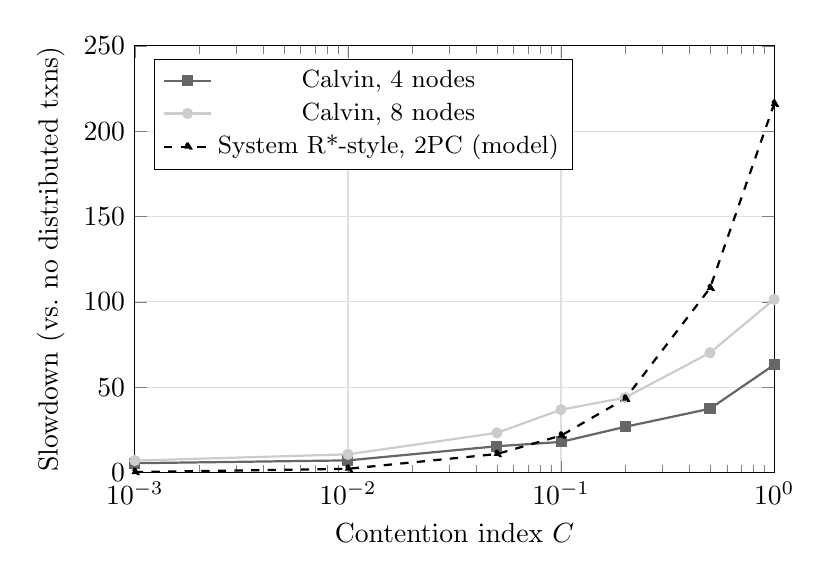
\begin{tikzpicture}
\begin{axis}[
  width=0.8\textwidth, height=7cm,
  xmode=log, xmin=0.001, xmax=1, ymin=0, ymax=250,
  xlabel={Contention index $\hot$}, ylabel={Slowdown (vs.\ no distributed txns)},
  grid=major, grid style={gray!25},
  legend style={at={(0.03,0.97)},anchor=north west,font=\small}]
\addplot[thick,color=calgrayB,mark=square*,mark size=1.6pt]
  coordinates {(0.001,5.42)(0.01,7.07)(0.05,15.36)(0.1,17.90)(0.2,26.74)(0.5,37.34)(1.0,63.08)};
\addlegendentry{Calvin, 4 nodes}
\addplot[thick,color=calgrayA,mark=*,mark size=1.6pt]
  coordinates {(0.001,6.96)(0.01,10.61)(0.05,23.20)(0.1,36.79)(0.2,43.86)(0.5,70.15)(1.0,101.41)};
\addlegendentry{Calvin, 8 nodes}
\addplot[thick,dashed,color=calblack,mark=triangle*,mark size=1.4pt]
  coordinates {(0.001,0.216)(0.01,2.16)(0.05,10.8)(0.1,21.6)(0.2,43.2)(0.5,108.0)(1.0,216.0)};
\addlegendentry{System R*-style, 2PC (model)}
\end{axis}
\end{tikzpicture}
\caption{Reconstructed Figure~6. The 2PC model is
$\text{slowdown} = \num{27000}\cdot\hot\cdot D_{2PC}$ with
$D_{2PC}\approx\si{8} ms$.}
\label{fig:fig6}
\end{figure}

The 2PC reference is a deliberately generous \emph{lower bound} on
disadvantage: it ignores multipartition CPU cost, local commit/abort decision
latency, and execution-progress skew (it even assumes perfect lockstep
execution). Its derivation: at most $1/\hot$ transactions may run
concurrently, so a 2PC system commits at most $1/(\hot D_{2PC})$ per second,
with $D_{2PC} = 2\times\si{2} ms = \si{4} ms$ per hop, two hops.

\paragraph{Reading the comparison honestly.}
\begin{itemize}[leftmargin=1.2em,itemsep=2pt]
\item Crossover by log-linear interpolation: Calvin-4-node overtakes the 2PC
      model at $\hot \approx 0.08$; Calvin-8-node at $\hot \approx 0.56$.
\item Below $\hot\approx0.05$, a System R*-style system would be
      \emph{faster} than Calvin. The advantage materialises only in the
      high-contention multipartition regime --- which is precisely the
      argument the paper advances for why production systems abandon
      distributed ACID transactions.
\item The comparison is at $n=4$ and $n=8$ only; no 2PC curve is shown for
      Figure~5's $n\le100$ range.
\end{itemize}

% =====================================================================
\section{Caveats and limitations}
\label{sec:caveats}

\begin{enumerate}[leftmargin=1.6em,itemsep=3pt]
\item \textbf{``Scales linearly'' is conditional.} It is demonstrated for
      $\hot\le10^{-4}$ within $n\le100$. At $\hot=10^{-2}$ the per-node
      curve is still falling $3\times$ over $10\to100$ nodes
      (\num{14578} $\to$ \num{4745}); only the \emph{marginal} contribution
      is roughly constant there.
\item \textbf{Real anti-scaling exists in the data.} For $\rho=1$,
      $\hot=10^{-4}$: \num{25948} txn/s at $n=1$ $\to$ \num{10265} at
      $n=2$. Two nodes are worse than one; it takes $\approx6$ nodes just to
      break even with a single node. Non-monotonic, and not highlighted in
      the paper.
\item \textbf{The $n=1$ baseline is not like-for-like.} At $n=1$ no
      multipartition transaction is executable, so the 1-node point contains
      no distributed-transaction cost at all. Part of the celebrated
      ``$1\to2$ drop'' is therefore the \emph{activation} of the distributed
      workload, not the cost of scale-out.
\item \textbf{Platform heterogeneity.} The paper notes all three Figure~5
      curves drop between 6 and 8 nodes, attributed to a slow EC2 instance
      joining the set. This contaminates $\approx5\,\%$ of the curve.
\item \textbf{The 2PC comparison is a model, not a measurement}, and the
      paper explicitly declines to call it a comparison point: it is
      ``somewhat na\"{\i}ve''.
\item \textbf{Latency is traded away.} All these runs add
      $\approx\si{5} ms$ of sequencer batching on the critical path, plus
      one remote round trip per multipartition transaction. The paper's
      scalability results are throughput results; Figure~2 shows replication
      across three continents (100--170\,ms ping) leaves throughput
      unaffected while inflating latency.
\item \textbf{Model honesty.} With two free parameters fit to $\approx10$
      digitised points, the $R^2$ values in Table~\ref{tab:fit} are \emph{not}
      independent validation --- $D(n)$ is a reparameterisation of $\pernode$.
      The non-circular content is (i) the falsification test of
      \S\ref{sec:pernode}, which uses only the paper's own latency floor;
      (ii) the $\rho$-linearity falsification of \S\ref{sec:rhonl}, which is
      internal to the data and needs no external assumption; and (iii) the
      capture of the $\rho{=}1,\ n{=}2$ anti-scaling point. The
      single-$D$ form does \emph{not} fit small-$n$ behaviour
      ($\approx\num{7300}$ predicted vs.\ \num{5268} measured at $n=2$,
      $\rho=1$); \eqref{eq:corrected} splits the penalty into a barrier floor
      and a saturating skew term to address this.
\item \textbf{The model is falsified in its simplest form.} \eqref{eq:cost}
      assumes $c_m - c_s$ is linear in $\rho$. Table~\ref{tab:rhonl} shows it
      is not: $\gRatio$ runs from \num{1.561} at $n{=}2$ to \num{0.924} at
      $n{=}100$. Any $D$ fit to a single $\rho$ therefore carries an
      unquantified systematic error, which is why the $1/\hot$ exponents in
      \S\ref{sec:oneoverC} should be read as descriptive only.
\item \textbf{$\nueff$ is unidentified.} $c_s=\SI{307}{\msecs}$ is derived
      as $8/\pernode(1)$, which presumes CPU saturation. A single sequencer
      thread at \SI{38.3}{\msecs}/txn fits the same datum
      (\S\ref{sec:nueff}). Until CPU and sequencer-thread utilisation are
      measured, the model's asymptote is known only up to this factor, and the
      two hypotheses disagree about whether added cores help at all.
\item \textbf{The codebase is not the measured system.} All code citations
      refer to the later geo-replicated CalvinDB repository, which post-dates
      the SIGMOD~'12 prototype and adds a replication dimension
      (\texttt{MRSP}/\texttt{MRMP} transaction types) that the paper's
      experiments do not exercise. Structural facts (per-partition hot set,
      \texttt{SP}/\texttt{MP} split, local lock filtering, local commit
      validation) are lineage evidence and very likely correct; specific costs
      are not transferable.
\end{enumerate}

% =====================================================================
\section{Conclusions}

\begin{enumerate}[leftmargin=1.6em,itemsep=3pt]
\item \textbf{Aggregate-linear, per-node-sublinear.} Per-node throughput
      degrades to an asymptote; total throughput then grows linearly in $n$
      with constant marginal contribution (curve~A: \num{13684}\,$\pm$\SI{1}{\percent}
      txn/s per added node across $n=10\to100$).
\item \textbf{The knee is a fixed cost.} Remote-read serialisation, context
      switching and per-participant set-up/teardown are paid once and
      amortised; they do not grow with $n$.
\item \textbf{Determinism imposes order, not a lock.} The pairwise per-record
      constraint leaves disjoint-record transactions fully parallel, so there
      is no global serialisation point --- and no global ceiling.
\item \textbf{Contention is per machine.} $H = 1/\hot$ is a per-node window;
      the global window is $n/\hot$. The global reading is falsified by a
      factor of $5.5\times$, and the window is only \SI{1}{\percent}--\SI{19}{\percent}
      utilised in every measured configuration. Because the benchmark client is
      open-loop, this is structural, not accidental: the system never chooses to
      exceed the window.
\item \textbf{``Distributed'' is not a type, it is a key-set property.} Nothing
      in the system branches on it. The participant set is computed once
      centrally for routing and role assignment; the commit decision is purely
      local and uncoordinated. Being distributed therefore costs
      \num{8.9}--\num{17.3}$\times$ the local work it saves --- and the cost is
      dominated by a single \emph{barrier}, not by per-key serialisation.
\item \textbf{The penalty is not linear in $\rho$.} $\gRatio$ runs
      \num{1.561} $\to$ \num{0.924} as $n$ goes $2\to100$, crossing unity near
      $n\approx8$. The mechanism is partner correlation: at $n=2$ there is
      exactly one partner and the waits are perfectly correlated; at
      $n\gtrsim20$ there are enough independent partners to average out. This
      also explains the unremarked anti-scaling at $n=2$, $\rho=1$.
\item \textbf{The residual $n$-dependence is execution-progress skew}, and it is
      the \emph{only} genuinely $n$-dependent term. Its magnitude $D_\infty$ and
      saturation scale $n_0$ both appear to grow as $1/\hot$ --- qualitatively
      explaining why the $\hot=10^{-2}$ plateau has not been reached at $n=100$ ---
      but that exponent is estimated from only two contention levels and is
      partly confounded with the $\rho$ non-linearity above. Treat it as
      descriptive.
\item \textbf{There is a second, non-CPU ceiling.} The sequencer leader routes
      every transaction through \emph{one} thread, deserialising, hashing,
      re-serialising and copying it into $\bar k = 1+\rho$ sub-batches. Bounded at
      $\lesssim\SI{76}{\msecs}$ per extra participant. It does not bind at
      $n=2$ (<10\% of node cost) but is within a factor $\approx8$ of binding,
      and it caps $\pernode$ independently of core count --- which the
      CPU-capacity form of the model cannot express.
\end{enumerate}

\paragraph{What would settle the remaining questions.} (i) Report CPU and
sequencer-thread utilisation: this alone resolves $\nueff$ and therefore whether
added cores help. (ii) Run $\rho\in\{0,0.1,0.5,1\}$ at fixed $\hot$, giving
$3\times$ more $\rho$ points and de-contaminating the $1/\hot$ exponent.
(iii) Constrain the partner to a fixed small pool at $n=8$; $\gRatio\approx1.5$
would confirm the correlation mechanism. (iv) Extend curve~C past $n=100$ to
observe the predicted $n\approx84$--$130$ plateau directly. Each of these is a
single-figure experiment.

% =====================================================================
\appendix
\section{Digitisation procedure and validation}
\label{app:method}

\paragraph{Method.} For each figure page, the PDF content stream was parsed for
path operators (\texttt{m}, \texttt{l}) together with stroke-colour operators
(\texttt{SC}); consecutive operators were grouped into polylines, one per data
series. Axes were calibrated from the plot-frame rectangle and tick marks
present in the same stream, and cross-validated against tick-label glyph
bounding boxes. Legend entries were bound to series by exploiting the emission
order in the stream: gnuplot emits a legend key line immediately followed by
its polyline, so the $n$th key pairs with the $n$th polyline.

\paragraph{Note on a tooling pitfall.} \texttt{pdfplumber} reports coordinates
for XObject content that are displaced by a non-constant offset (e.g.\ the
Figure~4 total-throughput curve is reported at $y=72.1$ where the raw stream
gives $y=719.9$). Calibrating against pdfplumber coordinates therefore yields
plausible-looking but wrong values. The raw content streams were parsed
directly to avoid this.

\paragraph{Validation against the paper's prose.}

\begin{table}[H]
\centering
\begin{tabular}{@{}lll@{}}
\toprule
\textbf{Quantity} & \textbf{Paper states} & \textbf{Extracted} \\
\midrule
100-node TPC-C total & ``nearly half a million'' & \num{440971} \\
TPC-C per-node, $n>10$ & ``around \num{5000} per node'' & \num{4475}--\num{5524} \\
1-node microbenchmark & ``about \num{27000} per second per machine'' & \num{25948} \\
Fig.~6 low-contention, 4 nodes & ``\ldots{}to about \num{5000}'' & \num{4986} \\
Fig.~6 low-contention, 8 nodes & ``\ldots{}or \num{4000}'' & \num{3879} \\
Per-node $= $ total/$n$ & (not stated) & holds to $\le\SI{0.5}{\percent}$ \\
\bottomrule
\end{tabular}
\end{table}

\paragraph{Full digitised series.} All coordinates are given in
Tables~\ref{tab:fig4}, \ref{tab:fig5} and \ref{tab:fig6}. Curves~B in
Figure~5 omits the $n=60$ and $n=80$ x-values in the published figure itself;
this is a property of the original plot, not of the extraction.

% =====================================================================
\section{Provenance of the code citations}
\label{app:code}

Every \srcfile{} reference in \S\ref{sec:whatis}, \S\ref{sec:seq} and
\S\ref{sec:nueff} is to the repository at
\texttt{/home/otrack/tmp/calvindb}, lines as of the analysis date.

\begin{table}[H]
\centering
\caption{Lineage caveat: this is the \emph{later} geo-replicated CalvinDB, not
the SIGMOD~'12 prototype measured in the paper. The thread structure cited in
\S\ref{sec:seq} is therefore evidence about design lineage, not a direct
measurement of the system in Figure~5. Two concrete divergences from the paper:
\texttt{MicroTxnSP} uses $2$ hot keys where the paper describes $1$, and the
modern build adds a deliberate CPU spin (120\,$\msecs$ per factor,
\texttt{factor} $=2.0$ for multipartition) that is not a Calvin cost.}
\label{tab:provenance}
\begin{tabular}{@{}>{\raggedright\arraybackslash}p{5.3cm}
                  >{\raggedright\arraybackslash}p{5.0cm}
                  >{\raggedright\arraybackslash}p{\dimexpr\textwidth-10.3cm-4\tabcolsep\relax}@{}}
\toprule
\textbf{File:line} & \textbf{Role in this analysis} & \textbf{Reliance} \\
\midrule
\srcfile{sequencer.cc:119} &
  open-loop batch filling (\S\ref{sec:pernode}) &
  structural \\
\srcfile{sequencer.cc:187} &
  participant computation, fan-out ceiling (\S\ref{sec:seq}) &
  structural \\
\srcfile{microbenchmark.cc:55} &
  \texttt{MicroTxnSP}: $2$ hot $+$ cold, all local &
  quantitative \\
\srcfile{microbenchmark.cc:101} &
  \texttt{MicroTxnMP}: $2$ hot across two partitions &
  quantitative \\
\srcfile{microbenchmark.cc:473} &
  \texttt{txn\_type} read \ldots{} only here &
  structural \\
\srcfile{microbenchmark.h} &
  $k_{\text{RW}}{}=10$, per-partition \texttt{hot\_records} &
  quantitative \\
\srcfile{client.h:57} &
  uniform-random partner: the $\rho$-mix knob &
  structural \\
\srcfile{calvindb_server.cc:25} &
  \texttt{-{}-percent\_mp}: the Figure~5 legend itself &
  direct \\
\srcfile{deterministic_lock_manager.cc:23} &
  \texttt{IsLocal(key)}: remote keys filtered before lock wait &
  structural \\
\srcfile{storage_manager.cc:172} &
  local commit revalidation, \texttt{size()==1} shortcut &
  structural \\
\bottomrule
\end{tabular}
\end{table}

\paragraph{How the paper's knobs map to flags.} The correspondence between the
Figure~5 legend and the implementation is direct enough to be treated as
certain: \texttt{--percent\_mp=10} \emph{is} ``10\% distributed txns'',
\texttt{--contention=10\^{}-4} sets \texttt{hot\_records}${}=10^{4}$ per
partition, and the $C$ of the paper is $1/\texttt{hot\_records}$. The
per-machine scoping of $C$ --- the result of \S\ref{sec:pernode} --- is thus
visible in a single line of the generator:

\begin{lstlisting}[language=C]
hotkey = part + nparts * (rand() % hot_records);
\end{lstlisting}

The hot set is indexed \emph{within} a partition, so every node presents an
independent window of $H=\texttt{hot\_records}$ records. There is no global
window anywhere in the system.

\paragraph{Negative result.} A tree-wide search for \texttt{txn\_type} returns
hits under \srcfile{src/applications/} and \srcfile{src/scripts/} only. Neither
\srcfile{src/machine/}, \srcfile{src/scheduler/}, \srcfile{src/backend/} nor
\srcfile{src/log/} reads it. This is the basis for the claim in
\S\ref{sec:whatis} that ``distributed'' is not a runtime type, and it is the
one code claim that would be falsified by a single reference outside
\texttt{src/applications/}.

\end{document}